\chapter{UNIQUE HARDWARE CHARACTERISTICS OF A MOBILE DEVICE}\label{cha:character}\index{characteristics}
In the hardware of a device there are some features that can be used to distinguish devices from each other. In the pyramid below showing features from a mobile device that can be used for fingerprinting a device. This chapter will cover explanation on why and how this can be done for the sensors and radio signal.
\begin{figure}[!h]
		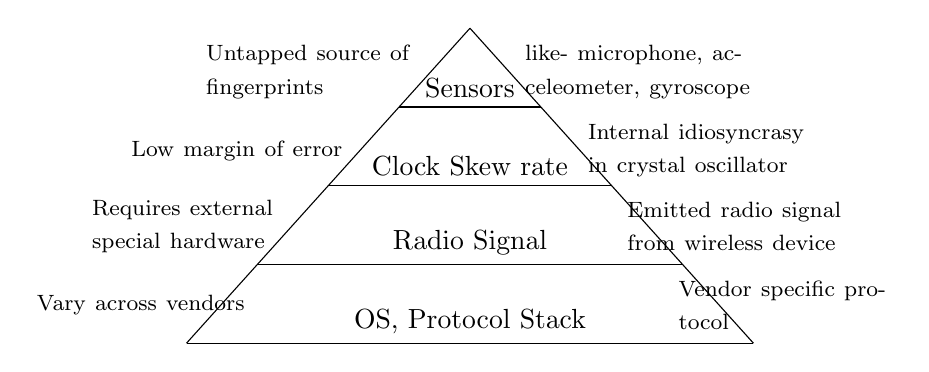
\begin{tikzpicture}[scale=1]

		\def \h {4};
		\def \f {0.9};

		\foreach \y in  {0,1,2,3} {
		    \def \w { \h*\f-\y*\f };
		    \def \v { \y*\f-\h*\f };
		    \draw (\v,\y) -- (\w,\y);
		}

		\draw (-\h*\f,0)  -- (0,\h);
		\draw (\h*\f,0)  -- (0,\h);
		\node (os) at (0,0) [above] {OS, Protocol Stack};
		\node (rf) at (0,1) [above] {Radio Signal};
		\node (cs) at (0,2) [above] {Clock Skew rate};
		\node (se) at (0,3) [above] {Sensors};


		\node [left of=os, xshift=-3cm, yshift=0.2cm, text width=3cm] {\footnotesize{Vary across vendors}};
		\node [left of=rf, xshift=-2.4cm, yshift=0.2cm, text width=2.8cm] {\footnotesize{Requires external special hardware}};
		\node [left of=cs, xshift=-1.8cm, yshift=0.2cm, text width=3cm] {\footnotesize{Low margin of error}};
		\node [left of=se, xshift=-1cm, yshift=0.2cm, text width=2.7cm] {\footnotesize{Untapped source of fingerprints}};

		\node [right of=os, xshift=3cm, yshift=0.2cm, text width=2.7cm] {\footnotesize{Vendor specific protocol}};
		\node [right of=rf, xshift=2.5cm, yshift=0.2cm, text width=3cm] {\footnotesize{Emitted radio signal from wireless device}};
		\node [right of=cs, xshift=2cm, yshift=0.2cm, text width=3cm] {\footnotesize{Internal idiosyncrasy in crystal oscillator}};
		\node [right of=se, xshift=1.2cm, yshift=0.2cm, text width=3cm] {\footnotesize{like- microphone, acceleometer, gyroscope}};
	\end{tikzpicture}
	\caption{\label{fig:pyramid} The pyramid of features in a mobile device that can be used for fingerprinting.\cite[]{sensor:acoustic}}
\end{figure}
The clock skew rate will not be covered in this thesis because it is proven REFERENSER!! not to be unique enough for authentication purposes.The bottom layer of the pyramid, OS and protocol stack will not be covered since it vary across vendors and has vendor specific protocols that will be out of the time frame to look in to.

\section{Sensors}\label{sec:sensors}\index{sensor}
As seen above in~\figureref{fig:pyramid} are sensors an untapped source of fingerprints in mobile devices and example of sensors are microphone, accelerometer, barometer, speakers and gyroscope. In this chapter will accelerometer, gyroscope, microphone and speaker sensors in mobile devices be presented and how collecting characteristic noise from them is done.

\subsection{Accelerometer\index{accelerometer}}\label{sec:accelerometer}
The accelerometer is the sensor that detect movement on a mobile device, like when you changing orientation on your device. Acceleration is measured by sensing how much pressure the device has in terms of force. A mobile device in rest relative to the surface of the earth has about 1G\index{G} (gravitational-force). \cite[]{sensors:allref}\\
In mobile devices is done using a micro-electro-mechanical system (MEMS\index{MEMS}) that translates electrical property-changes (as voltage) and translated into signals. Processing is then done by software in the mobile device. Mobile devices today uses three different accelerometers; \textit{micro-electromechanical system} that reacts when forces affect them which is changing an electrical property. \textit{Capacitive accelerometer} reacts when a net force is applied on the mechanical system, that is resulting a change in capacitance. The \textit{piezoelectric accelerometer} uses as the name implies the structures of piezoelectric crystals. These are crystals that reacts on forces applied to the mobile device trough creating electrical charges that generate voltage. 
\url{http://www.techopedia.com/definition/24430/accelerometer} \\
\\
Measure the error characteristics from the accelerometer is done by taking the long term average of the output when the accelerometer is in rest. That is the biggest error source in the accelerometer and it grows quadratically over time, but when the accelerometer is in rest the error $epsilon$ can be calculated as a function of time $t$;
$$s(t)=\epsilon * \frac{t^2}{2} $$
\cite[]{sensor:inertialNav}\\
\\


\subsection{Gyroscope\index{gyroscope}}\label{sec:gyroscope}
The gyroscope is sensing how the device is moving in terms of angles, for maintaining or measure the orientation. This is originally  a mechanical system based on the principle of conservation of angular momentum. The most popular Gyroscope for devices today is a MEMS that is using silicon micro-mechanical techniques. Coriolis effect is measured with vibrating elements in the MEMS gyroscope. Coriolis effect is a change of moving objects direction when looking at it from a rotating reference system. The difference from the accelerometer is that the gyroscope measures relative to the device body rather than relative to earth. The equations of Coriolis force;  
$$\boldsymbol{ F}_C = -2 \, m \, (\omega *  v)$$
Where $m$ is the mass of the particle, $\omega$ the angular velocity and $v$ the velocity of the particle in the rotating system. 
\cite[]{sensor:inertialNav} \\
\\
The MEMS sensors is common used because has many pros such small (like a hair), light, cheap, low powered, etc. The MEMS gyro is also known for high reliability but it has some error characteristics like constant bias, white noise, bias instability, calibration error and temperature effects. One of these error characteristics that can be tested by reading the output from a gyroscope in rest is the \\\textit{constant bias}\index{constant bias}. That is bias of the gyroscope output when not having any rotation on it. This constant error $\epsilon$ of the bias over time $t$ leads to an angular error that grows linear; 
$$\theta (t)= \epsilon * t $$
If take the long term average output from the gyro in rest, the constant error of a rate gyro can be estimated.  


\subsection{Microphone \& Speaker}\label{sec:char:micSpeak}\index{microphone}
A microphone or speaker on a mobile device is like accelerometer and gyroscope a MEMS. Today mobile devices has one, two or three MEMS microphone. When a sound reaches the microphone sets a diaphragm in motion by the pressure from the sound wave. The motion causes capacitive change and that leads to a change of voltage. In short terms is the pressure of the sound converted to electrical signals. \cite[]{sensor:acoustic}\\
A normalized output gain over a given frequency range is the response from a microphone that has specification in a \index{frequency response graph} frequency response graph.The range should ideally be the same as for the speaker. In the real world however the response curve varies between different frequencies, depending on the design of the mobile device.  \cite[]{sensor:micSpek}\\
\\ 
The error characteristics in the microphone or speaker due to inconsistent in the manufacturing. This inconsistencies does that not even microphones of the same model are identical. Every manufacturer of microphones and speaker specifies a tolerance for these errors and it is typical $\pm$2db.  \cite[]{sensor:micSpek}

\subsection{Camera}\label{sec:char:camera}\index{camera fingerprinting}\index{camera}
The digital camera of a mobile device also includes sensors and other hardware that can be used as fingerprinting characteristics. The basic is that light travels trough a lens and hits a imaging sensor which contains pixels that has a filter array in front. The filter is for gives each pixel a detected color. The pixels is then put together again to a resulting signal which is send to some final post processing (color correction, white balance, etc.) steps before the image is written to the memory card. In this process there are different kind of noise that effects the image;
\begin{itemize}
	\item[] \textit{\index{shot noise}Shot noise -} the amount of photons hitting the sensor and each pixel varies a random amount
	\item[] \textit{\index{fixed pattern noise}Fixed pattern noise - }there is a small electric current that leaks from photo-diodes in each pixel, caused by dark current
	\item[] \textit{\index{photo-response non-uniformity noise}\index{PRNU}Photo-response non-uniformity noise (PRNU) -} is a noise that is not affected by temperature or humidity. When manufacturing sensors the silicon gets imperfection which causes that pixels aren't equally sensitive to light. This is the main source of pattern noise and makes it really unlikely for two cameras to have the same pattern.
\end{itemize}
The three types of noise can be described as a mathematical model for getting the output of the sensor $y_{ij}$:
$$y_{ij}=f_{ij}(x_{ij}+\eta_{ij})+c_{ij}+\epsilon_{ij}$$
where $f_{ij}$ is a multiple factor close to one that captures PRNU noise, $x_{ij}$ is the number of photons hitting the sensor, $\eta_{ij}$ the shot noise, $c_{ij}$ the dark current and $\epsilon_{ij}$ the additive random noise. The key for a unique fingerprint of the camera (in the mobile device) is to finding $f$.
\cite[]{sensor:camera:DCIdent}


\section{Clock skew rate}\label{sec:clockskew}\index{clock skew}
Mobile devices today have a lot of clocks both in hardware and software. These clocks isn't all that synced as you may think and have what is called a clock skew rate between them, which is the time difference between them. This could be a thing to measure as unique characteristics if the clocks always is equally wrong. \cite[]{clockSkew}\\
\\
Measuring the clock skew rate remotely is done by comparing different clocks from the device with a more correct clock, like an atomic clock.
In the paper~\cite[]{clockSkew} and... LÄGG TILL FLER KÄLLOR!! they conclude that the clock skew rate isn't unique enough for fingerprinting device. Due to that it's proven not completely unique it will not be good enough for a fingerprint and something the mobile devise \textit{are} in two-factor authentication purpose. 

\section{Radio signal}\label{sec:radiosignal}\index{radio signal}\index{RFF}
Wireless devices that want to connect to another device sends radio signals. This signals can be used for fingerprinting the device by passively analyzing radio-frequency\index{radio-frequency} (RF) in IEEE 802.11 and finding the source network interface card (\index{NIC}NIC) . Where you can find characteristic errors for each device due to transmitter-specific imperfections in the signal. There are different artifacts that can be taken into account for fingerprinting. This is known as radio frequency fingerprinting\index{radio frequency fingerprinting} (RFF\index{RFF}). \cite[]{rff:wifiDeviceSign}\\
\\


ish funkar \cite[]{rff:identWiFi} , \cite[]{rff:passiveDLLwifi}, \cite[]{rff:wifiDeviceSign}\\
\\
följt av ett stycke om hur man mäter bruset.